

%%%%%%%%%%%%%%%%%%%%%%%%%%%%%%%%%%%%%%%%%
% Journal Article
% LaTeX Template
% Version 1.4 (15/5/16)
%
% This template has been downloaded from:
% http://www.LaTeXTemplates.com
%
% Original author:
% Frits Wenneker (http://www.howtotex.com) with extensive modifications by
% Vel (vel@LaTeXTemplates.com)
%
% License:
% CC BY-NC-SA 3.0 (http://creativecommons.org/licenses/by-nc-sa/3.0/)
%
%%%%%%%%%%%%%%%%%%%%%%%%%%%%%%%%%%%%%%%%%

%----------------------------------------------------------------------------------------
%	PACKAGES AND OTHER DOCUMENT CONFIGURATIONS
%----------------------------------------------------------------------------------------

\documentclass[10pt]{article} % Single column

%\documentclass[twoside,twocolumn]{article} % Two column

\usepackage{blindtext} % Package to generate dummy text throughout this template 

\usepackage[sc]{mathpazo} % Use the Palatino font
\usepackage[T1]{fontenc} % Use 8-bit encoding that has 256 glyphs
\linespread{1.05} % Line spacing - Palatino needs more space between lines
\usepackage{microtype} % Slightly tweak font spacing for aesthetics

\usepackage[english]{babel} % Language hyphenation and typographical rules

\usepackage{algorithm}
	
\usepackage[hmarginratio=1:1,top=32mm,columnsep=20pt]{geometry} % Document margins
\usepackage[hang, small,labelfont=bf,up,textfont=it,up]{caption} % Custom captions under/above floats in tables or figures
\usepackage{booktabs} % Horizontal rules in tables

\usepackage{lettrine} % The lettrine is the first enlarged letter at the beginning of the text

\usepackage{enumitem} % Customized lists
\setlist[itemize]{noitemsep} % Make itemize lists more compact

\usepackage{abstract} % Allows abstract customization
\renewcommand{\abstractnamefont}{\normalfont\bfseries} % Set the "Abstract" text to bold
\renewcommand{\abstracttextfont}{\normalfont\small\itshape} % Set the abstract itself to small italic text

\usepackage{titlesec} % Allows customization of titles
\renewcommand\thesection{\Roman{section}} % Roman numerals for the sections
\renewcommand\thesubsection{\roman{subsection}} % roman numerals for subsections
\titleformat{\section}[block]{\large\scshape\centering}{\thesection.}{1em}{} % Change the look of the section titles
\titleformat{\subsection}[block]{\large}{\thesubsection.}{1em}{} % Change the look of the section titles

\usepackage{fancyhdr} % Headers and footers
\pagestyle{fancy} % All pages have headers and footers
\fancyhead{} % Blank out the default header
\fancyfoot{} % Blank out the default footer
\fancyhead[C]{Alternative Topic Modeling Optative Course. \textbf{Study of LDA Method}} % Custom header text
\fancyfoot[RO,LE]{\thepage} % Custom footer text

\usepackage{titling} % Customizing the title section

\usepackage{hyperref} % For hyperlinks in the PDF

\usepackage{graphicx} % For images

\usepackage{pifont} % bullets

\usepackage{amsmath}

\usepackage{algpseudocode}

\usepackage{lipsum}

% Keywords command
\providecommand{\keywords}[1]
{
	\small	
	\vspace{0.5em}
	\noindent \textbf{\textit{Keywords --- }} #1
}


%----------------------------------------------------------------------------------------
%	TITLE SECTION
%----------------------------------------------------------------------------------------

\setlength{\droptitle}{-4\baselineskip} % Move the title up

\pretitle{\begin{center}\Huge\bfseries} % Article title formatting
	\posttitle{\end{center}} % Article title closing formatting
\title{\normalsize{Alternative Topic Modeling Optative Course}\\
	\Huge\bfseries Study of LDA Method \\
} % Article title
\author{% 
	Laura Victoria Riera P\'erez\\
	Mari\'e del Valle Reyes \vspace{1em} \\
	\small Senior year. Computer Science. \\ % institution
	\small School of Math and Computer Science, University of Havana, Cuba \\ % institution
}
\date{\footnotesize \today } % Leave empty to omit a date


% Abstract configurations
\renewenvironment{abstract}
{\small
	\begin{center}
		\bfseries \abstractname\vspace{-.5em}\vspace{0pt}
	\end{center}
	\list{}{
		\setlength{\leftmargin}{1.5cm}%
		\setlength{\rightmargin}{\leftmargin}%
	}%
	\item\relax}
{\endlist}

\usepackage{amsthm}
\usepackage{amssymb}
\usepackage{todonotes} % \TODO
\usepackage{listings} % Code listings
\usepackage{xcolor}

\definecolor{backcolour}{rgb}{0.95,0.95,0.92}

\newcommand{\csl}[1]{\colorbox{backcolour}{\texttt{#1}}}

\newcommand{\imgcaption}[2]{\tiny \textbf{Figura #1.} #2.}

\newcommand{\mgc}[2][]{\colorbox{backcolour}{\texttt{\_\_#2\_\_#1}}}

\newcommand{\mgccapt}[1]{\texttt{\_\_#1\_\_}}

\newtheorem{thm}{Teorema}
\newtheorem{mydef}{Definici\'on}%[section]
\newtheorem{lem}{Lema}
\newtheorem{fig}{\scriptsize{Figura}}
\newtheorem{col}{Corolario}


\renewcommand{\qedsymbol}{\rule{0.7em}{0.7em}}

% Hyperlinks configurations
\hypersetup{
	colorlinks=true,
	linkcolor=black,
	filecolor=magenta,      
	urlcolor=cyan,
	pdftitle={Overleaf Example},
	pdfpagemode=FullScreen,
}

%----------------------------------------------------------------------------------------

\begin{document}
	% Print the title
	\maketitle
	
	%----------------------------------------------------------------------------------------
	%	ARTICLE CONTENTS
	%----------------------------------------------------------------------------------------
	\begin{abstract}
		\lipsum[1]
		
		\keywords{}
	\end{abstract}

	\section*{Project's repository}
	
	\begin{center}
		\href{https://github.com/computer-science-crows/study-of-lda-method}{https://github.com/computer-science-crows/study-of-lda-method}
	\end{center}
	
	\section{Initial Analysis}
	
	\subsection{Different coherence and perplexity}
	
	En el modelo de LDA (Latent Dirichlet Allocation), la coherencia y la perplexity pueden variar cuando se ejecuta el modelo varias veces con el mismo conjunto de palabras. Esto se debe a la naturaleza estocástica del algoritmo y a los diferentes factores que pueden influir en los resultados.
	
	\begin{center}
		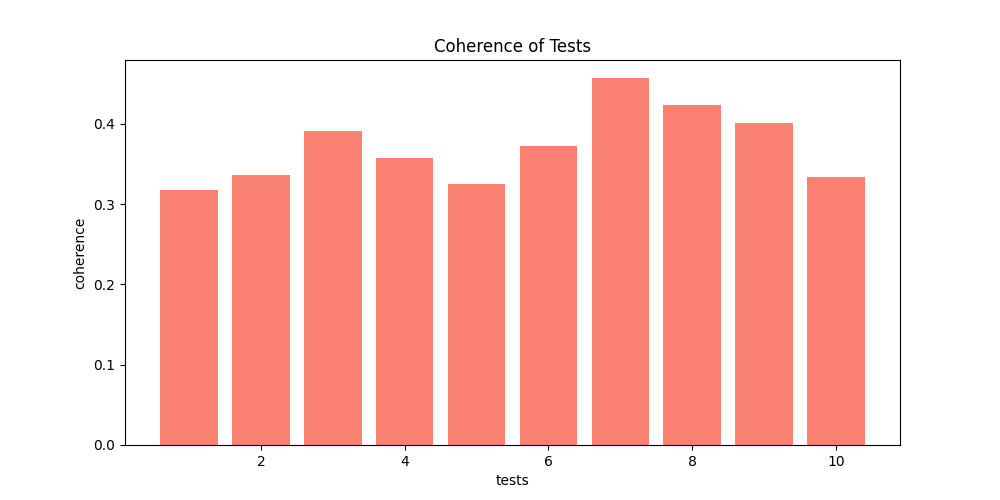
\includegraphics[scale=0.6]{images/coherence_stopwords}
		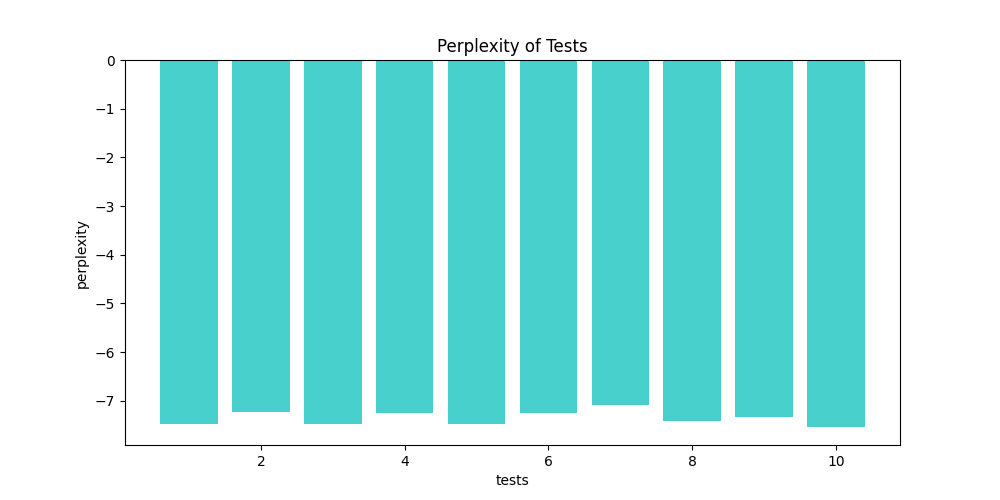
\includegraphics[scale=0.6]{images/perplexity_stopwords}
	\end{center}
	
	La perplexity es una medida utilizada en los modelos de LDA para evaluar qué tan bueno es el modelo en términos de ajuste a los datos. Cuanto más bajo sea el valor de la perplexity, mejor será el ajuste del modelo. Sin embargo, la perplexity puede variar entre diferentes ejecuciones del modelo debido a la inicialización aleatoria y a la forma en que se generan los temas y se asignan las palabras. Por lo tanto, es posible que obtengas diferentes valores de perplexity cada vez que ejecutes el modelo con el mismo conjunto de palabras.
	
	La coherencia, por otro lado, es una medida que evalúa cuánta coherencia tienen los temas generados por el modelo. La coherencia se basa en la relación entre las palabras dentro de cada tema y se utiliza para determinar qué tan interpretables son los temas. Al igual que con la perplexity, la coherencia también puede variar en diferentes ejecuciones del modelo debido a la aleatoriedad y a otros factores.
	
	La variabilidad en la coherencia y la perplexity puede deberse a varios factores, como la inicialización aleatoria del modelo, la selección de parámetros, la calidad del corpus de entrenamiento y la cantidad de datos disponibles. Además, diferentes implementaciones de LDA pueden tener variaciones en la forma en que se calcula la coherencia y la perplexity, lo que también puede contribuir a las diferencias en los resultados.
	
	Es importante tener en cuenta que tanto la coherencia como la perplexity son medidas aproximadas y no proporcionan una evaluación definitiva de la calidad del modelo de LDA. Se deben utilizar en conjunto con otras técnicas de evaluación y análisis para obtener una comprensión más completa de los resultados del modelo.
	
	En resumen, la coherencia y la perplexity pueden variar cuando se ejecuta el modelo de LDA varias veces con el mismo conjunto de palabras debido a la aleatoriedad y a otros factores involucrados en el algoritmo. Es importante considerar estas variaciones y utilizar otras técnicas de evaluación para obtener una imagen más completa de la calidad del modelo
	
	\subsection{Solution}
	
	Para solucionar el problema de la variabilidad en la coherencia y perplexity en el modelo LDA al ejecutarlo múltiples veces con el mismo conjunto de palabras, se pueden considerar las siguientes estrategias:
	\begin{enumerate}
		\item Ajustar los parámetros del modelo: Los parámetros del modelo LDA, como el número de temas y las iteraciones de entrenamiento, pueden influir en los resultados. Es posible que ajustar estos parámetros pueda mejorar la coherencia y perplexity. Puedes experimentar con diferentes valores y evaluar cómo afectan los resultados.
		
		\item Utilizar una semilla aleatoria fija: La inicialización aleatoria del modelo puede ser una fuente de variabilidad en los resultados. Al establecer una semilla aleatoria fija antes de cada ejecución del modelo, puedes asegurarte de que las inicializaciones sean consistentes y obtener resultados más estables.
		
		\item 	Aumentar la cantidad de datos de entrenamiento: La cantidad de datos de entrenamiento también puede afectar la estabilidad de los resultados. Si tienes un conjunto de palabras pequeño, es posible que la variabilidad sea mayor. Considera agregar más datos o ampliar el corpus de entrenamiento para obtener resultados más consistentes.
		
		\item Realizar promedios de múltiples ejecuciones: En lugar de confiar en los resultados de una sola ejecución del modelo, puedes realizar múltiples ejecuciones y promediar los resultados. Esto puede ayudar a reducir la variabilidad y obtener una estimación más confiable de la coherencia y perplexity.
		
		\item Utilizar técnicas de validación cruzada: La validación cruzada es una técnica que puede ayudar a evaluar el rendimiento del modelo en diferentes particiones del conjunto de datos. Al realizar validación cruzada, puedes obtener una medida más robusta de la coherencia y perplexity, ya que se evalúa el modelo en diferentes subconjuntos de datos.
	\end{enumerate}
	
	Es importante tener en cuenta que, aunque estas estrategias pueden ayudar a reducir la variabilidad en la coherencia y perplexity, es posible que aún exista cierta variación en los resultados. Esto se debe a la naturaleza estocástica del algoritmo y a la complejidad inherente de los datos de texto. Es recomendable evaluar los resultados de múltiples ejecuciones y utilizar otras técnicas de evaluación para obtener una comprensión más completa del modelo LDA.
	
	\subsection{Test 8}
	
	La mayoria de las palabras son stopwords.
	
	\begin{center}
		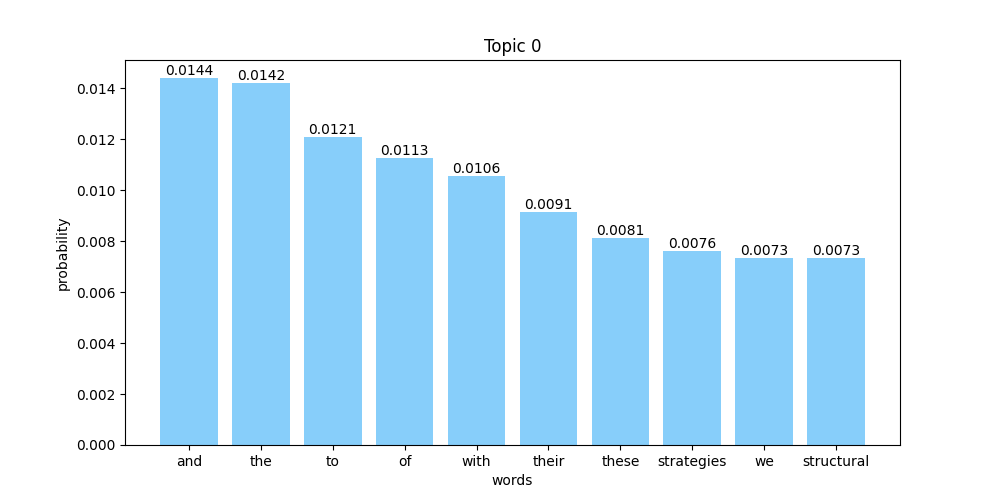
\includegraphics[scale=0.6]{images/plots/test_8/topic_0.png}
		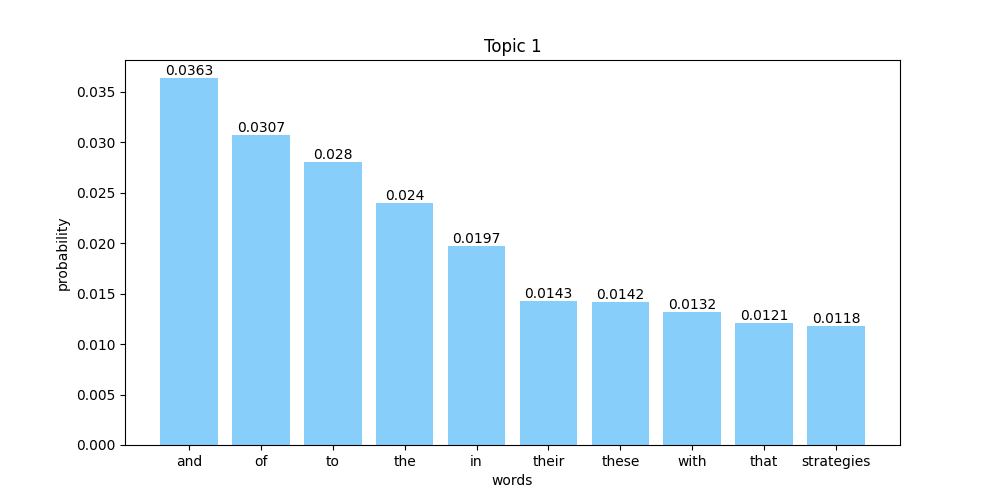
\includegraphics[scale=0.6]{images/plots/test_8/topic_1.png}
		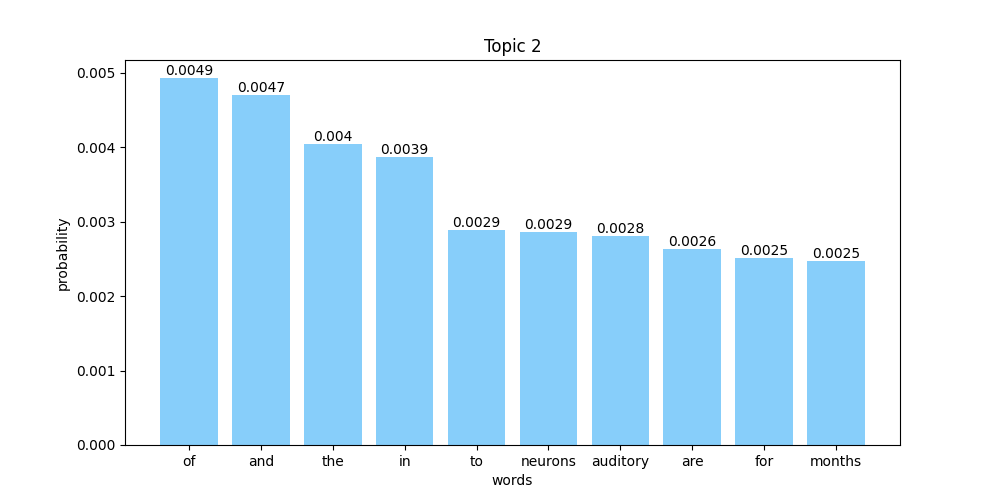
\includegraphics[scale=0.6]{images/plots/test_8/topic_2.png}
		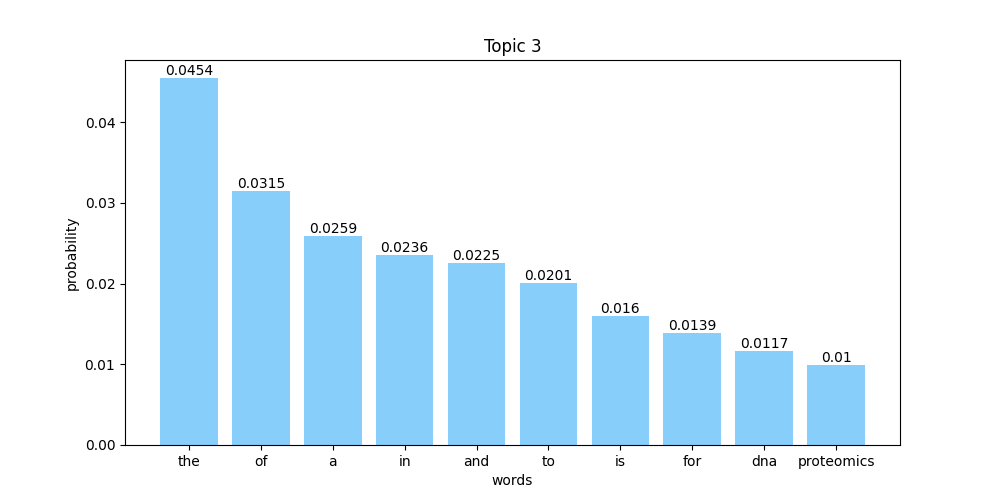
\includegraphics[scale=0.6]{images/plots/test_8/topic_3.png}
		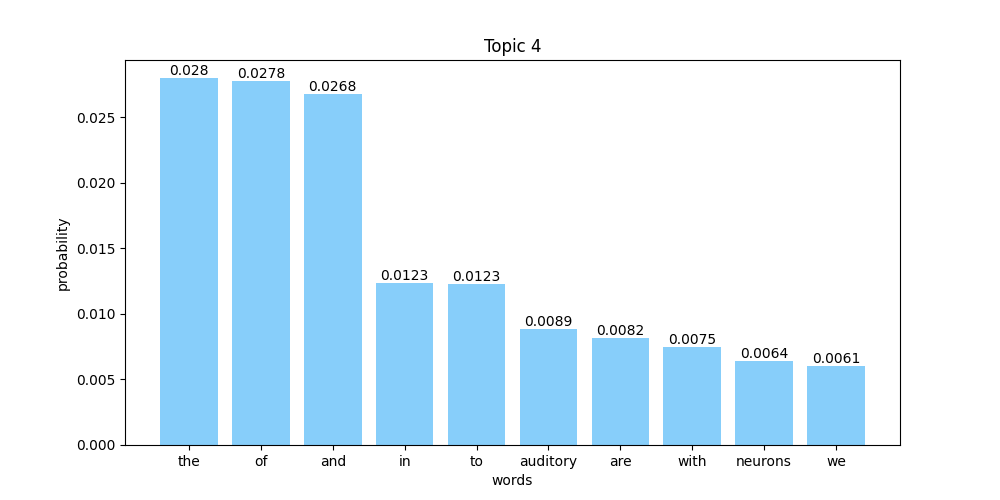
\includegraphics[scale=0.6]{images/plots/test_8/topic_4.png}\\
		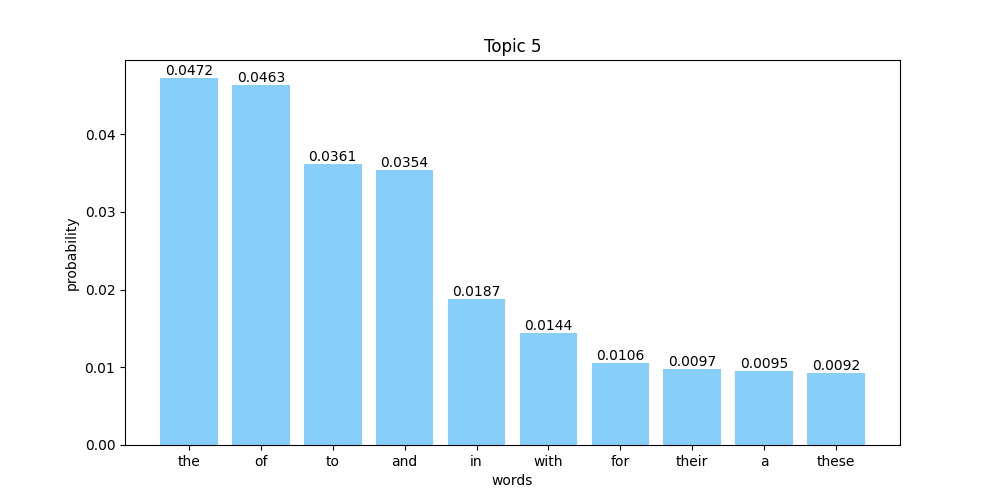
\includegraphics[scale=0.6]{images/plots/test_8/topic_5.png}
		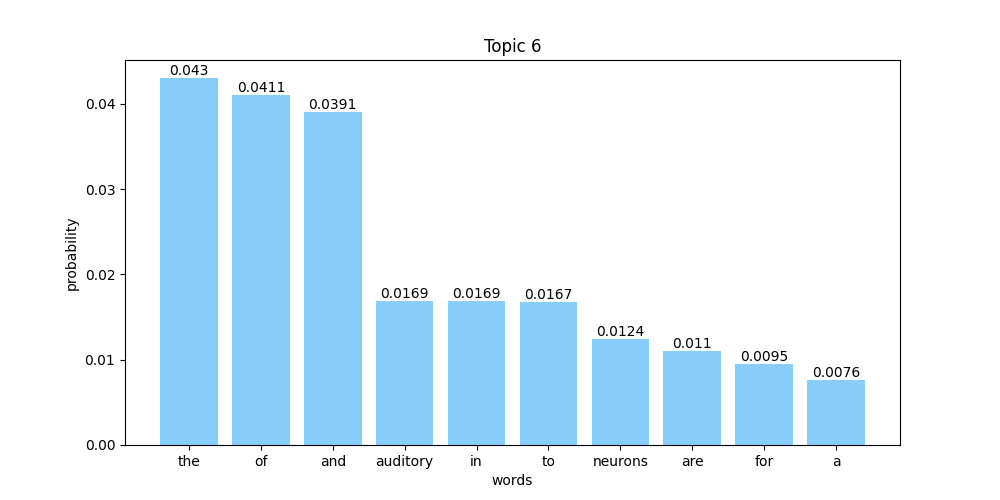
\includegraphics[scale=0.6]{images/plots/test_8/topic_6.png}
		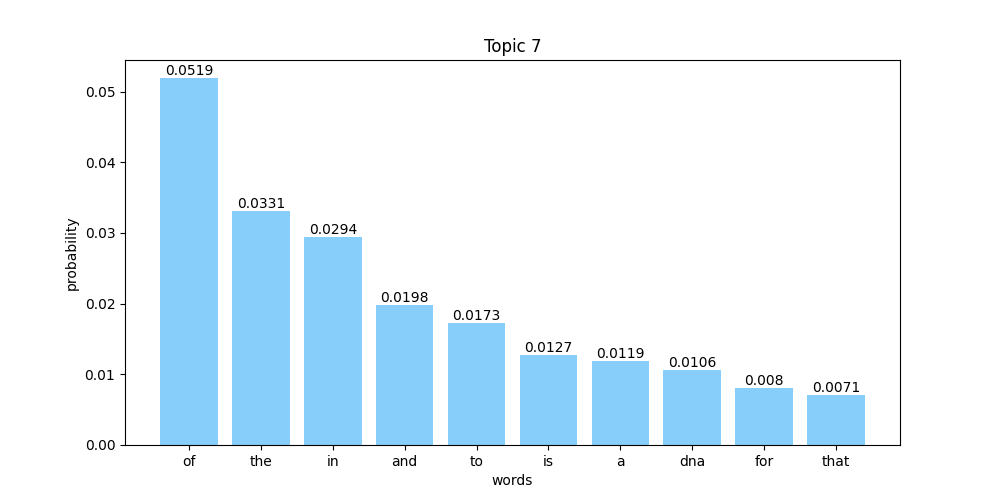
\includegraphics[scale=0.6]{images/plots/test_8/topic_7.png}
	\end{center}

	La perplexity es -7.255103257328984, y la coherencia  0.3718197713201331.
	
	
	\section{Removing stopwords}
	
	La eliminación de las stopwords (palabras vacías) es un paso común en la preparación de datos para el modelado de tópicos con LDA. Las stopwords son palabras muy comunes y frecuentes en un idioma determinado, como "el", "y", "de", "a", etc. Estas palabras no aportan mucho significado o información relevante para la identificación de temas y pueden afectar negativamente la calidad de los resultados de LDA.
	
	Aquí hay algunas razones por las que se deben remover las stopwords al realizar LDA:
	\begin{enumerate}
		\item Reducción del ruido: Al eliminar las stopwords, se reduce el ruido en los datos. Las stopwords son palabras tan comunes que aparecen en casi todos los documentos y no proporcionan información distintiva sobre los temas. Al eliminarlas, se reduce la cantidad de palabras irrelevantes en el análisis y se enfoca en las palabras más significativas para la identificación de tópicos.
		
		\item 	Mejor interpretación de tópicos: Al eliminar las stopwords, se mejora la interpretabilidad de los tópicos generados por el modelo de LDA. Las stopwords tienden a aparecer en múltiples tópicos y no ayudan a distinguir claramente los temas. Al eliminarlas, se destacan las palabras clave más relevantes y distintivas de cada tópico, lo que facilita su interpretación y análisis.
		
		\item Reducción de la dimensionalidad: Al eliminar las stopwords, se reduce la dimensionalidad del espacio de palabras utilizado para el modelado de tópicos. Esto puede ayudar a mejorar la eficiencia computacional y reducir el consumo de memoria. Al eliminar palabras muy frecuentes pero poco informativas, se puede lograr una representación más compacta y eficiente de los documentos.
	\end{enumerate}
	
	La eliminación de las stopwords se puede realizar utilizando listas predefinidas de stopwords específicas de cada idioma. Estas listas contienen palabras comunes que se consideran stopwords y se pueden encontrar fácilmente en línea. Por ejemplo, para el idioma español, puedes encontrar listas de stopwords que contienen palabras como "el", "y", "de", etc.
	
	En resumen, la eliminación de stopwords en el proceso de LDA es importante para reducir el ruido en los datos, mejorar la interpretación de los tópicos y reducir la dimensionalidad del espacio de palabras. Esto ayuda a obtener resultados más precisos y significativos en el modelado de tópicos con LDA
	
	\subsection{Stopwords}
	
	Stop words are commonly used words in a language that are often considered insignificant or carry little meaning in the context of natural language processing (NLP) and text mining. These words are typically articles, prepositions, conjunctions, or pronouns. Examples of stop words in English include "a", "the", "is", "are", and so on. Stop words are used to eliminate words that are so commonly used that they may not contribute much to the analysis or understanding of text data.
	
	\subsection{Code Modification}
	
	Se creo un nuevo .py en donde se descomentaron las lineas de c\'odigo que se encargaban de eliminar las stopwords del conjunto de palabras dado en TokenVieuxM.txt.
	
	\begin{center}
		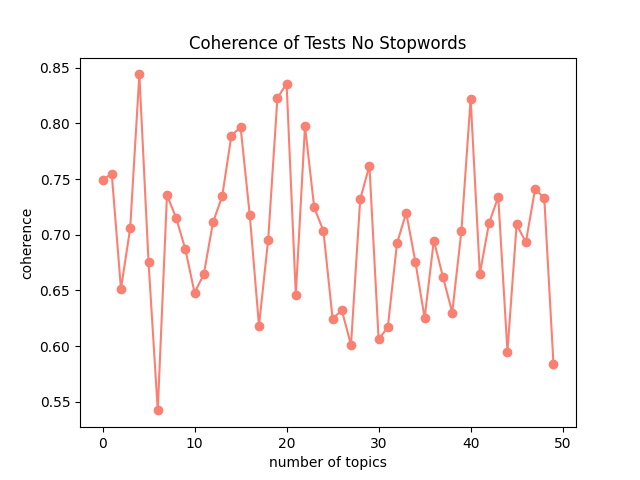
\includegraphics[scale=0.6]{images/coherence_no_stopwords}
		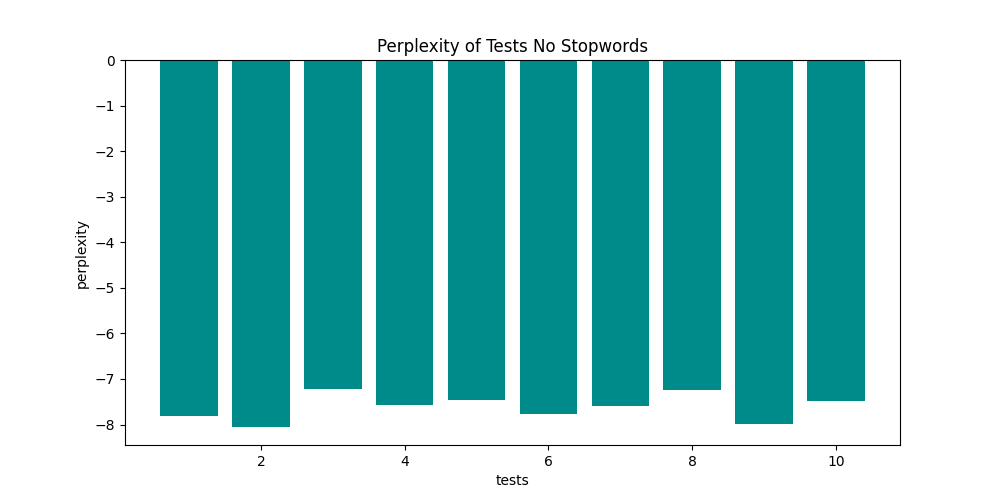
\includegraphics[scale=0.6]{images/perplexity_no_stopwords}
	\end{center}

	\subsubsection{Test 8 No Stopwords}
	
	\begin{center}
		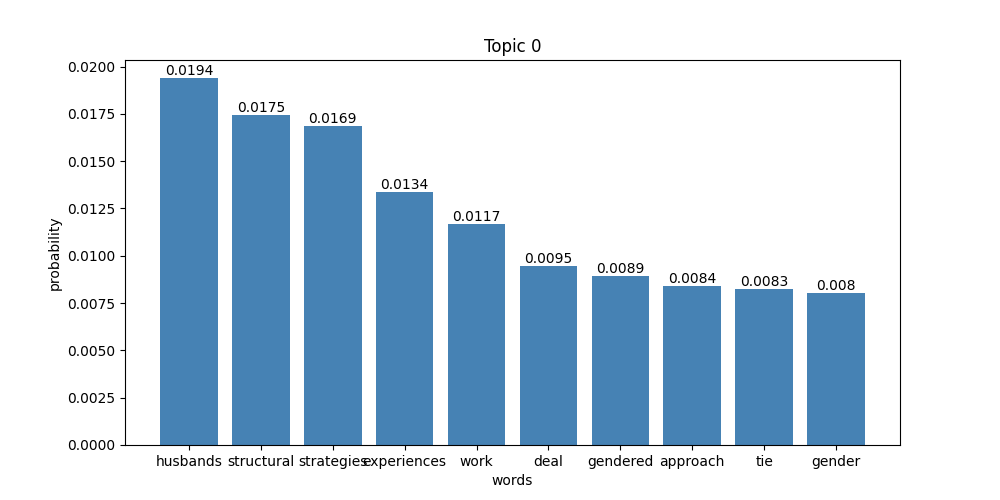
\includegraphics[scale=0.6]{images/plots/test_8_no_stopwords/topic_0.png}
		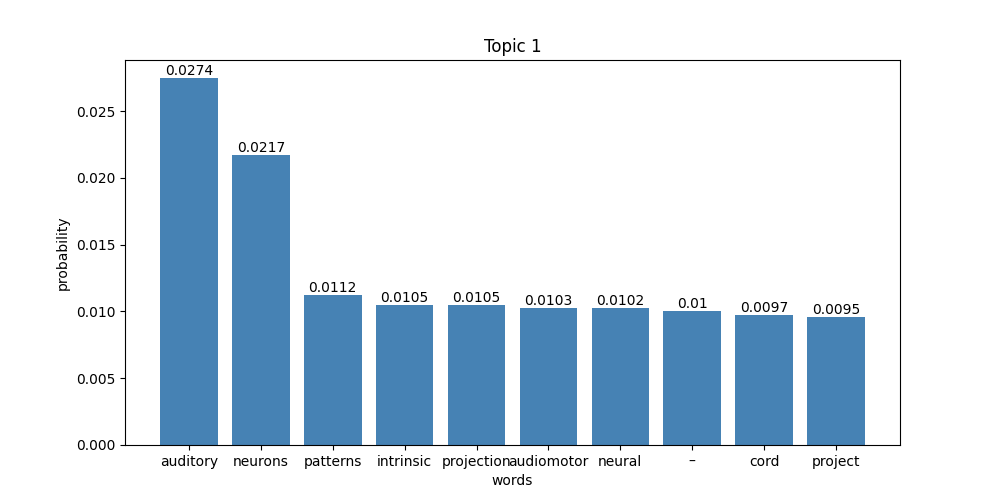
\includegraphics[scale=0.6]{images/plots/test_8_no_stopwords/topic_1.png}
		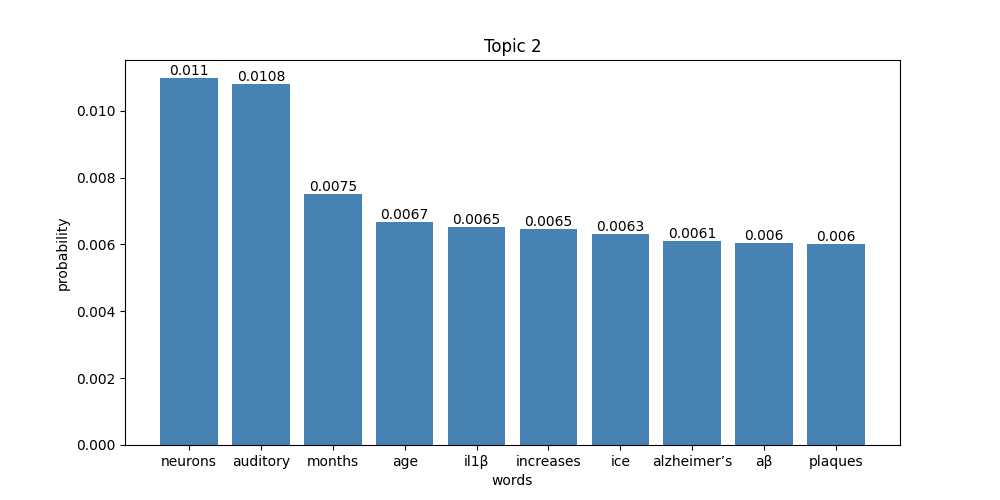
\includegraphics[scale=0.6]{images/plots/test_8_no_stopwords/topic_2.png}
		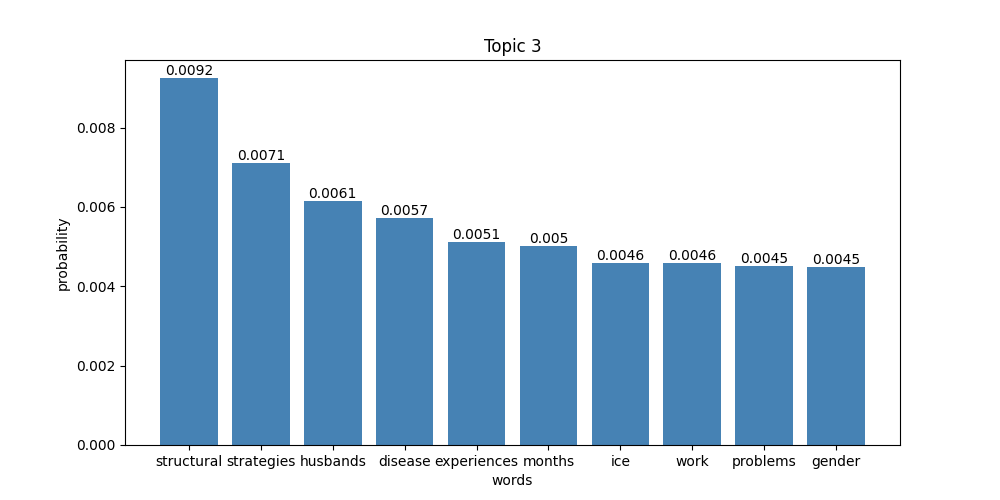
\includegraphics[scale=0.6]{images/plots/test_8_no_stopwords/topic_3.png}\
		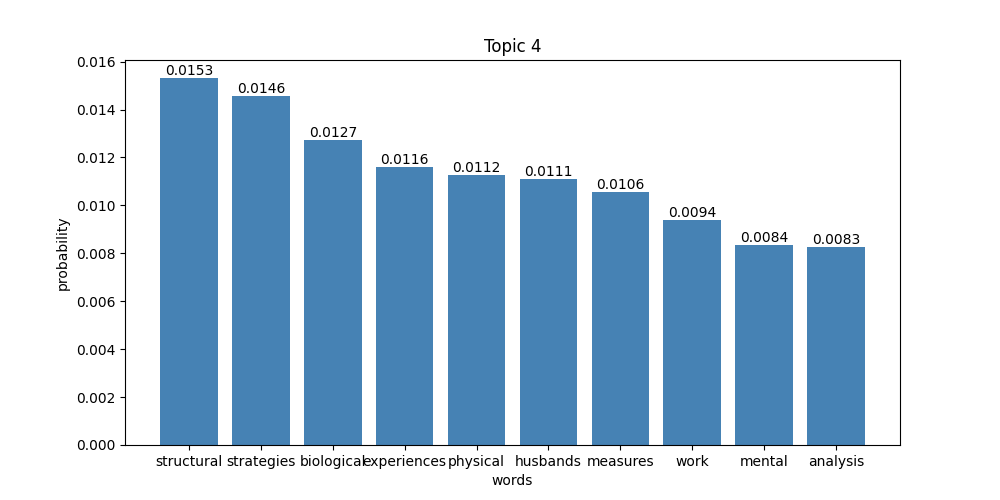
\includegraphics[scale=0.6]{images/plots/test_8_no_stopwords/topic_4.png}
		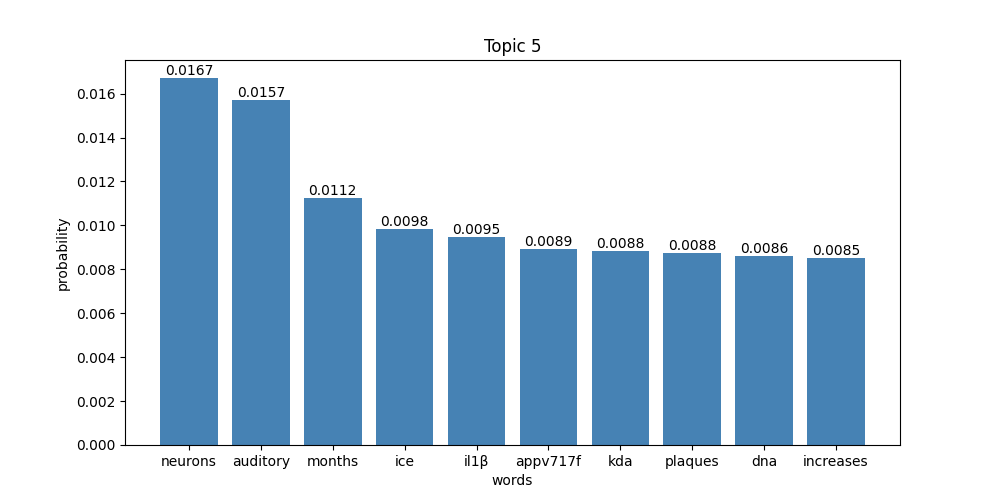
\includegraphics[scale=0.6]{images/plots/test_8_no_stopwords/topic_5.png}
		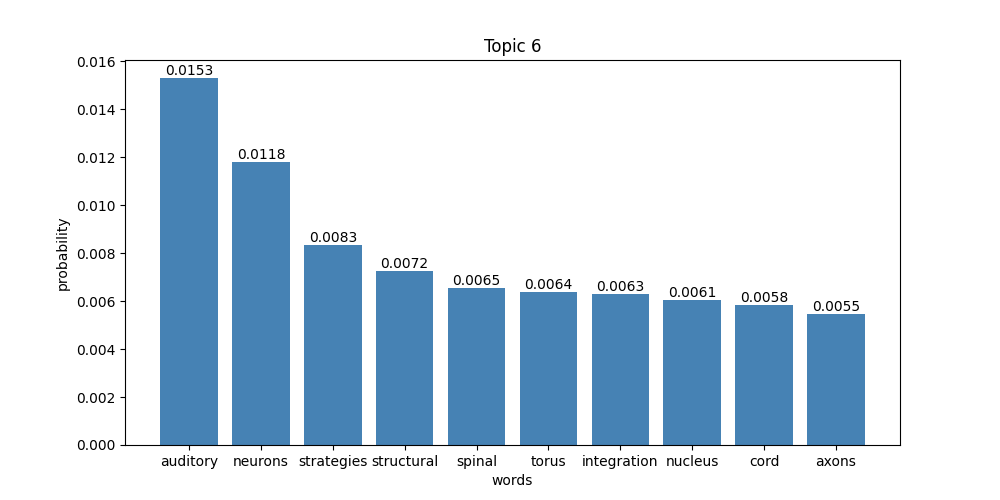
\includegraphics[scale=0.6]{images/plots/test_8_no_stopwords/topic_6.png}
		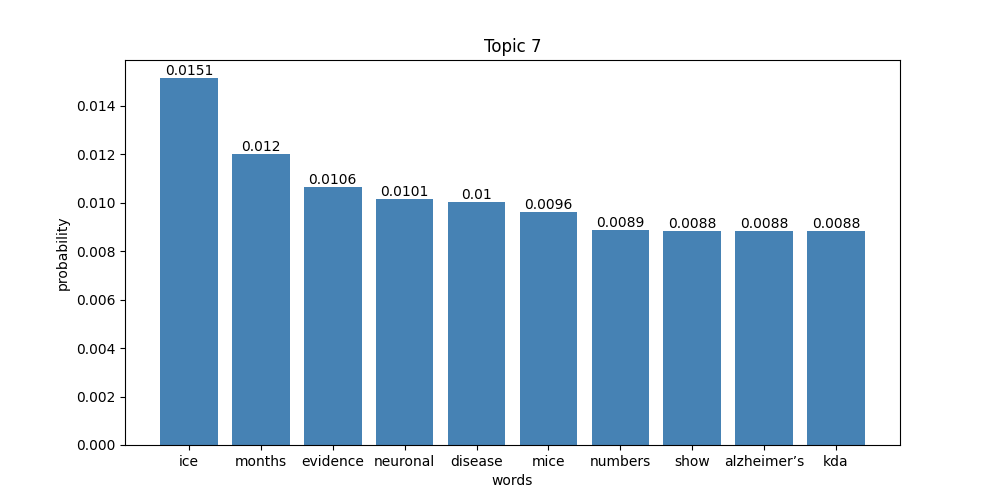
\includegraphics[scale=0.6]{images/plots/test_8_no_stopwords/topic_7.png}
		
		
	\end{center}

	La perplexity es -7.764361092424768 y la coherencia  0.6284575950301475.

	\todo{hay que comparar los resultados con el test sin remover stopwords y ver la relaci\'on entre coherencia y perplexity}
	
	\subsection{Changing number of topics}
	
	\begin{center}
		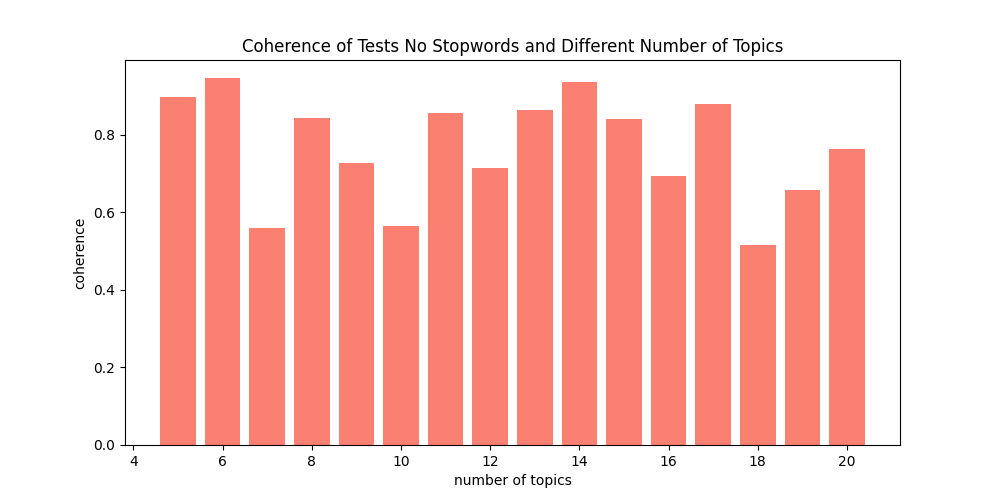
\includegraphics[scale=0.6]{images/coherence_no_stopwords_diff_n_topics}
		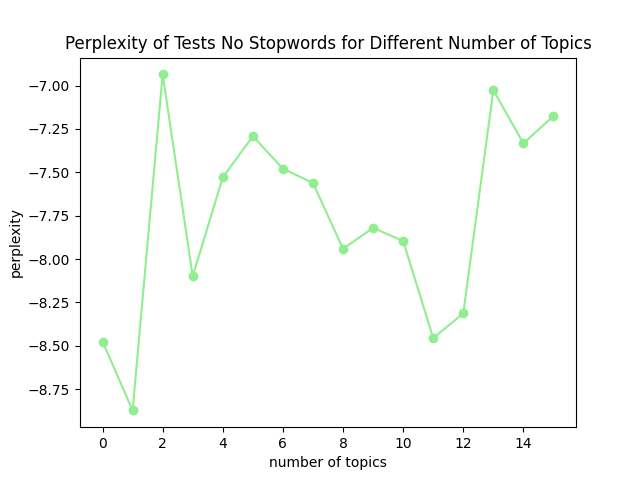
\includegraphics[scale=0.6]{images/perplexity_no_stopwords_diff_n_topics}
	\end{center}

	El n\'umero \'optimo de t\'opicos de acurdo a los valores de coherencias deber\'ia ser 6.
	
	\todo{falta plotear los test con el otro dataset}
	
	\section{Most typical documents for topics}
	
	Para identificar el documento más típico en cada tópico utilizando LDA de Gensim en Python, puedes utilizar el método get\_document\_topics proporcionado por la clase LdaModel. Este método devuelve una lista de tuplas que contienen el ID del tópico y la probabilidad de ese tópico para cada documento.
	
	
	
	\begin{thebibliography}
		a
		\bibitem{introduction} Cormen, Thomas H. y otros. \emph{Introduction to Algorithms}. 
		The MIT Press.
		4ta Edici\'on.		
		Cambridge, Massachusetts.
		2022.
	\end{thebibliography}
\end{document}


